\chapter{Graphics including GenomeDiagram}
\label{chapter:graphics}

The \verb|Bio.Graphics| module depends on the third party Python library
\href{http://www.reportlab.org}{ReportLab}.  Although focused on producing PDF files,
ReportLab can also create encapsulated postscript (EPS) and (SVG) files.  In addition
to these vector based images, provided certain further dependencies such as the
\href{http://www.pythonware.com/products/pil/}{Python Imaging Library (PIL)} are
installed, ReportLab can also output bitmap images (including JPEG, PNG, GIF, BMP
and PICT formats).

\section{GenomeDiagram}
\label{sec:genomediagram}
\subsection{Introduction}

The \verb|Bio.Graphics.GenomeDiagram| module was added to Biopython 1.50,
having previously been available as a separate Python module dependent on Biopython.
GenomeDiagram is described in the Bioinformatics journal publication by Pritchard et al. (2006) \cite{pritchard2006},
which includes some examples images. There is a PDF copy of the old manual here,
\url{http://biopython.org/DIST/docs/GenomeDiagram/userguide.pdf} which has some
more examples.
%TODO - Leighton's old website is AWOL, put this link back later if possible.
%http://bioinf.scri.ac.uk/lp/programs.php#genomediagram

As the name might suggest, GenomeDiagram was designed for drawing whole genomes, in
particular prokaryotic genomes, either as linear diagrams (optionally broken up into
fragments to fit better) or as circular wheel diagrams.  Have a look at Figure 2 in
Toth \textit{et al.} (2006) \cite{toth2006}
for a good example. It proved also well suited to drawing quite detailed figures for
smaller genomes such as phage, plasmids or mitochrondia, for example see Figures 1
and 2 in Van der Auwera \textit{et al.} (2009) \cite{vanderauwera2009}
(shown with additional manual editing).

This module is easiest to use if you have your genome loaded as a \verb|SeqRecord|
object containing lots of \verb|SeqFeature| objects - for example as loaded from a
GenBank file (see Chapters~\ref{chapter:SeqRecord} and~\ref{chapter:Bio.SeqIO}).

\subsection{Diagrams, tracks, feature-sets and features}

GenomeDiagram uses a nested set of objects.  At the top level, you have a diagram
object representing a sequence (or sequence region) along the horizontal axis (or
circle).  A diagram can contain one or more tracks, shown stacked vertically (or
radially on circular diagrams).  These will typically all have the same length
and represent the same sequence region.  You might use one track to show the gene
locations, another to show regulatory regions, and a third track to show the GC
percentage. %Talk about cross-links here? Maybe better later...

The most commonly used type of track will contain features, bundled together in
feature-sets.  You might choose to use one feature-set for all your CDS features,
and another for tRNA features.  This isn't required - they can all go in the same
feature-set, but it makes it easier to update the properties of just selected
features (e.g. make all the tRNA features red).

There are two main ways to build up a complete diagram.  Firstly, the top down
approach where you create a diagram object, and then using its methods add
track(s), and use the track methods to add feature-set(s), and use their
methods to add the features.  Secondly, you can create the individual objects
separately (in whatever order suits your code), and then combine them.

\subsection{A top down example}
\label{sec:gd_top_down}

We're going to draw a whole genome from a \verb|SeqRecord| object read in from
a GenBank file (see Chapter~\ref{chapter:Bio.SeqIO}).  This example uses the
pPCP1 plasmid from \textit{Yersinia pestis biovar Microtus}, the file is
included with the Biopython unit tests under the GenBank folder, or online
\href{http://biopython.org/SRC/biopython/Tests/GenBank/NC_005816.gb}
{\texttt{NC\_005816.gb}} from our website.

\begin{verbatim}
from reportlab.lib import colors
from reportlab.lib.units import cm
from Bio.Graphics import GenomeDiagram
from Bio import SeqIO
record = SeqIO.read("NC_005816.gb", "genbank")
\end{verbatim}

We're using a top down approach, so after loading in our sequence we next
create an empty diagram, then add an (empty) track, and to that add an
(empty) feature set:

\begin{verbatim}
gd_diagram = GenomeDiagram.Diagram("Yersinia pestis biovar Microtus plasmid pPCP1")
gd_track_for_features = gd_diagram.new_track(1, name="Annotated Features")
gd_feature_set = gd_track_for_features.new_set()
\end{verbatim}

Now the fun part - we take each gene \verb|SeqFeature| object in our
\verb|SeqRecord|, and use it to generate a feature on the diagram. We're
going to color them blue, alternating between a dark blue and a light blue.
\begin{verbatim}
for feature in record.features:
    if feature.type != "gene":
        #Exclude this feature
        continue
    if len(gd_feature_set) % 2 == 0:
        color = colors.blue
    else:
        color = colors.lightblue
    gd_feature_set.add_feature(feature, color=color, label=True)
\end{verbatim}

Now we come to actually making the output file.  This happens in two steps,
first we call the \verb|draw| method, which creates all the shapes using
ReportLab objects.  Then we call the \verb|write| method which renders these
to the requested file format.  Note you can output in multiple file formats:

\begin{verbatim}
gd_diagram.draw(format="linear", orientation="landscape", pagesize='A4',
                fragments=4, start=0, end=len(record))
gd_diagram.write("plasmid_linear.pdf", "PDF")
gd_diagram.write("plasmid_linear.eps", "EPS")
gd_diagram.write("plasmid_linear.svg", "SVG")
\end{verbatim}

Also, provided you have the dependencies installed, you can also do bitmaps,
for example:

\begin{verbatim}
gd_diagram.write("plasmid_linear.png", "PNG")
\end{verbatim}

\begin{htmlonly}
%The blank line below is important to start a new paragraph
\imgsrc[width=550, height=400]{images/plasmid_linear.png}

\end{htmlonly}
\begin{latexonly}
The expected output is shown in Figure~\ref{fig:plasmid_linear}.
\begin{figure}[htbp]
\centering
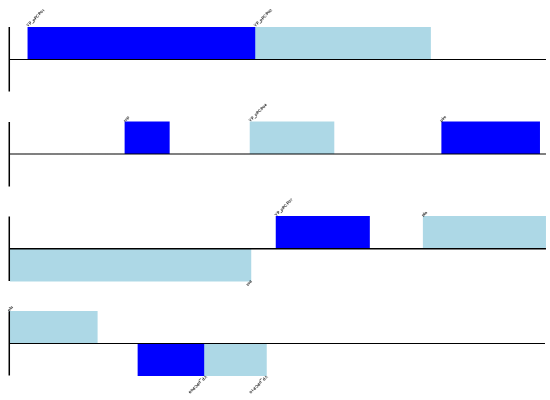
\includegraphics[width=0.8\textwidth]{images/plasmid_linear.png}
\caption{Simple linear diagram for \textit{Yersinia pestis biovar Microtus} plasmid pPCP1.}
\label{fig:plasmid_linear}
\end{figure}
\end{latexonly}
Notice that the \verb|fragments| argument which we set to four controls how
many pieces the genome gets broken up into.

If you want to do a circular figure, then try this:

\begin{verbatim}
gd_diagram.draw(format="circular", circular=True, pagesize=(20*cm,20*cm),
                start=0, end=len(record), circle_core=0.7)
gd_diagram.write("plasmid_circular.pdf", "PDF")
\end{verbatim}

\begin{htmlonly}
%The blank line below is important to start a new paragraph
\imgsrc[width=400, height=400]{images/plasmid_circular.png}

\end{htmlonly}
\begin{latexonly}
The expected output is shown in Figure~\ref{fig:plasmid_circular}.
\begin{figure}[htbp]
\centering
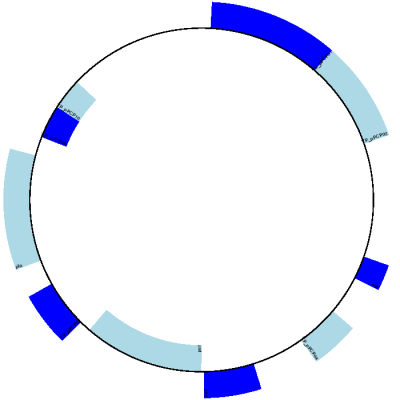
\includegraphics[width=8cm,height=8cm]{images/plasmid_circular.png}
\caption{Simple circular diagram for \textit{Yersinia pestis biovar Microtus} plasmid pPCP1.}
\label{fig:plasmid_circular}
\end{figure}
\end{latexonly}
These figures are not very exciting, but we've only just got started.

\subsection{A bottom up example}
Now let's produce exactly the same figures, but using the bottom up approach.
This means we create the different objects directly (and this can be done in
almost any order) and then combine them.

\begin{verbatim}
from reportlab.lib import colors
from reportlab.lib.units import cm
from Bio.Graphics import GenomeDiagram
from Bio import SeqIO
record = SeqIO.read("NC_005816.gb", "genbank")

#Create the feature set and its feature objects,
gd_feature_set = GenomeDiagram.FeatureSet()
for feature in record.features:
    if feature.type != "gene":
        #Exclude this feature
        continue
    if len(gd_feature_set) % 2 == 0:
        color = colors.blue
    else:
        color = colors.lightblue
    gd_feature_set.add_feature(feature, color=color, label=True)
#(this for loop is the same as in the previous example)

#Create a track, and a diagram
gd_track_for_features = GenomeDiagram.Track(name="Annotated Features")
gd_diagram = GenomeDiagram.Diagram("Yersinia pestis biovar Microtus plasmid pPCP1")

#Now have to glue the bits together...
gd_track_for_features.add_set(gd_feature_set)
gd_diagram.add_track(gd_track_for_features, 1)
\end{verbatim}

You can now call the \verb|draw| and \verb|write| methods as before to produce
a linear or circular diagram, using the code at the end of the top-down example
above.  The figures should be identical.

\subsection{Features without a SeqFeature}
\label{sec:gd_features_without_seqfeatures}

In the above example we used a \verb|SeqRecord|'s \verb|SeqFeature| objects
to build our diagram (see also Section~\ref{sec:seq_features}).
Sometimes you won't have \verb|SeqFeature| objects,
but just the coordinates for a feature you want to draw.  You have to create
minimal \verb|SeqFeature| object, but this is easy:

\begin{verbatim}
from Bio.SeqFeature import SeqFeature, FeatureLocation
my_seq_feature = SeqFeature(FeatureLocation(50,100),strand=+1)
\end{verbatim}

For strand, use \texttt{+1} for the forward strand, \texttt{-1} for the
reverse strand, and \texttt{None} for both.  Here is a short self contained
example:

\begin{verbatim}
from Bio.SeqFeature import SeqFeature, FeatureLocation
from Bio.Graphics import GenomeDiagram
from reportlab.lib.units import cm

gdd = GenomeDiagram.Diagram('Test Diagram')
gdt_features = gdd.new_track(1, greytrack=False)
gds_features = gdt_features.new_set()

#Add three features to show the strand options,
feature = SeqFeature(FeatureLocation(25, 125), strand=+1)
gds_features.add_feature(feature, name="Forward", label=True)
feature = SeqFeature(FeatureLocation(150, 250), strand=None)
gds_features.add_feature(feature, name="Strandless", label=True)
feature = SeqFeature(FeatureLocation(275, 375), strand=-1)
gds_features.add_feature(feature, name="Reverse", label=True)

gdd.draw(format='linear', pagesize=(15*cm,4*cm), fragments=1,
         start=0, end=400)
gdd.write("GD_labels_default.pdf", "pdf")
\end{verbatim}

\begin{htmlonly}
The top part of the image in the next subsection shows the output
\end{htmlonly}
\begin{latexonly}
The output is shown at the top of Figure~\ref{fig:gd_sigil_labels}
\end{latexonly}
(in the default feature color, pale green).

Notice that we have used the \texttt{name} argument here to specify the
caption text for these features.  This is discussed in more detail next.

\subsection{Feature captions}
\label{sec:gd_feature_captions}

Recall we used the following (where \texttt{feature} was a
\verb|SeqFeature| object) to add a feature to the diagram:

\begin{verbatim}
gd_feature_set.add_feature(feature, color=color, label=True)
\end{verbatim}

In the example above the \verb|SeqFeature| annotation was used to pick a
sensible caption for the features.  By default the following possible entries
under the \verb|SeqFeature| object's qualifiers dictionary are used:
\texttt{gene}, \texttt{label}, \texttt{name}, \texttt{locus\_tag}, and
\texttt{product}.  More simply, you can specify a name directly:

\begin{verbatim}
gd_feature_set.add_feature(feature, color=color, label=True, name="My Gene")
\end{verbatim}

In addition to the caption text for each feature's label, you can also choose
the font, position (this defaults to the start of the sigil, you can also
choose the middle or at the end) and orientation (for linear diagrams only,
where this defaults to rotated by $45$ degrees):

\begin{verbatim}
#Large font, parallel with the track
gd_feature_set.add_feature(feature, label=True, color="green",
                           label_size=25, label_angle=0)

#Very small font, perpendicular to the track (towards it)
gd_feature_set.add_feature(feature, label=True, color="purple",
                           label_position="end",
                           label_size=4, label_angle=90)

#Small font, perpendicular to the track (away from it)
gd_feature_set.add_feature(feature, label=True, color="blue",
                           label_position="middle",
                           label_size=6, label_angle=-90)
\end{verbatim}

\noindent Combining each of these three fragments with the complete example
in the previous section should give something like
\begin{htmlonly}
this:

%The blank lines above and below are important to trigger paragraph breaks
\imgsrc[width=600, height=700]{images/GD_sigil_labels.png}
\label{fig:gd_sigil_labels}

\end{htmlonly}
\begin{latexonly}
the tracks in Figure~\ref{fig:gd_sigil_labels}.
\begin{figure}[htbp]
\centering
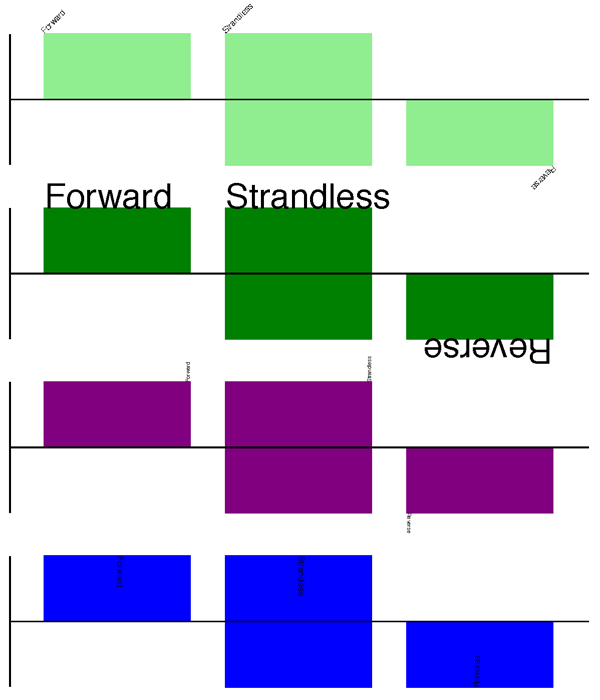
\includegraphics[width=0.8\textwidth]{images/GD_sigil_labels.png}
\caption{Simple GenomeDiagram showing label options.
The top plot in pale green shows the default label settings (see
Section~\ref{sec:gd_features_without_seqfeatures}) while the rest show
variations in the label size, position and orientation (see
Section~\ref{sec:gd_feature_captions}).
}
\label{fig:gd_sigil_labels}
\end{figure}
\end{latexonly}

We've not shown it here, but you can also set \texttt{label\_color} to
control the label's color (used in Section~\ref{sec:gd_nice_example}).

You'll notice the default font is quite small - this makes sense because
you will usually be drawing many (small) features on a page, not just a
few large ones as shown here.

\subsection{Feature sigils}
\label{sec:gd_sigils}

The examples above have all just used the default sigil for the feature, a
plain box, which was all that was available in the last publicly released standalone version of GenomeDiagram. Arrow sigils were included when
GenomeDiagram was added to Biopython 1.50:

\begin{verbatim}
#Default uses a BOX sigil
gd_feature_set.add_feature(feature)

#You can make this explicit:
gd_feature_set.add_feature(feature, sigil="BOX")

#Or opt for an arrow:
gd_feature_set.add_feature(feature, sigil="ARROW")
\end{verbatim}

\noindent
Biopython 1.61 added three more sigils,

\begin{verbatim}
#Box with corners cut off (making it an octagon)
gd_feature_set.add_feature(feature, sigil="OCTO")

#Box with jagged edges (useful for showing breaks in contains)
gd_feature_set.add_feature(feature, sigil="JAGGY")

#Arrow which spans the axis with strand used only for direction
gd_feature_set.add_feature(feature, sigil="BIGARROW")
\end{verbatim}

These are shown
\begin{htmlonly}
below.
\end{htmlonly}
\begin{latexonly}in Figure~\ref{fig:gd_sigils}.
\end{latexonly}
Most sigils fit into a bounding box (as given by the default BOX sigil),
either above or below the axis for the forward or reverse strand, or
straddling it (double the height) for strand-less features.
The BIGARROW sigil is different, always straddling the axis with the
direction taken from the feature's stand.

\begin{htmlonly}
\imgsrc[width=425, height=600]{images/GD_sigils.png}
\end{htmlonly}
\begin{latexonly}
\begin{figure}[htbp]
\centering
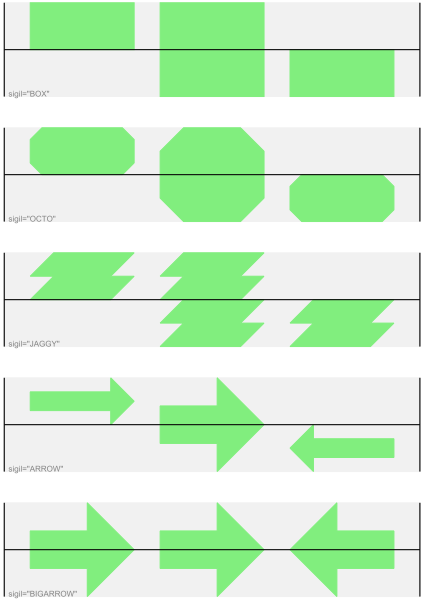
\includegraphics[width=0.8\textwidth]{images/GD_sigils.png}
\caption{Simple GenomeDiagram showing different sigils
(see Section~\ref{sec:gd_sigils})}
\label{fig:gd_sigils}
\end{figure}
\end{latexonly}

\subsection{Arrow sigils}
\label{sec:gd_arrow_sigils}

We introduced the arrow sigils in the previous section.
There are two additional options to adjust the shapes of the arrows, firstly
the thickness of the arrow shaft, given as a proportion of the height of the
bounding box:

\begin{verbatim}
#Full height shafts, giving pointed boxes:
gd_feature_set.add_feature(feature, sigil="ARROW", color="brown",
                           arrowshaft_height=1.0)
#Or, thin shafts:
gd_feature_set.add_feature(feature, sigil="ARROW", color="teal",
                           arrowshaft_height=0.2)
#Or, very thin shafts:
gd_feature_set.add_feature(feature, sigil="ARROW", color="darkgreen",
                           arrowshaft_height=0.1)
\end{verbatim}

\begin{htmlonly}
\noindent The results are shown below:

\imgsrc[width=600, height=700]{images/GD_sigil_arrow_shafts.png}

\end{htmlonly}
\begin{latexonly}
\noindent The results are shown in Figure~\ref{fig:gd_sigil_arrow_shafts}.
\begin{figure}[htbp]
\centering
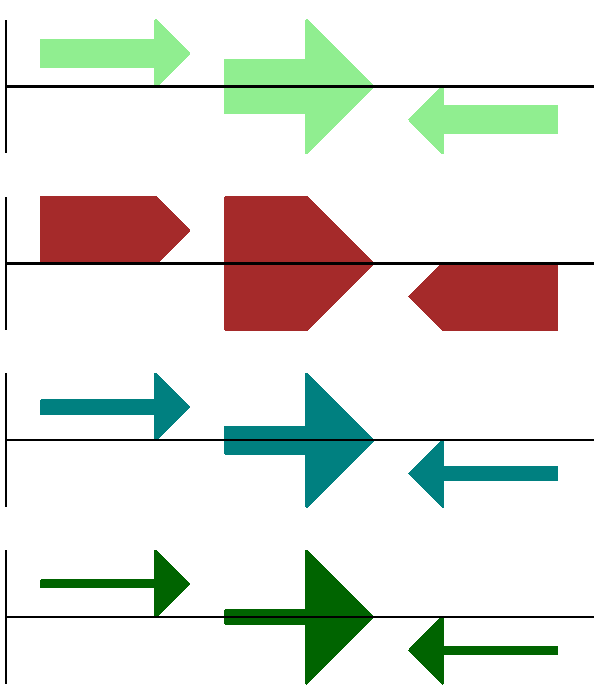
\includegraphics[width=0.8\textwidth]{images/GD_sigil_arrow_shafts.png}
\caption{Simple GenomeDiagram showing arrow shaft options
(see Section~\ref{sec:gd_arrow_sigils})}
\label{fig:gd_sigil_arrow_shafts}
\end{figure}
\end{latexonly}

Secondly, the length of the arrow head - given as a proportion of the height
of the bounding box (defaulting to $0.5$, or $50\%$):

\begin{verbatim}
#Short arrow heads:
gd_feature_set.add_feature(feature, sigil="ARROW", color="blue",
                           arrowhead_length=0.25)
#Or, longer arrow heads:
gd_feature_set.add_feature(feature, sigil="ARROW", color="orange",
                           arrowhead_length=1)
#Or, very very long arrow heads (i.e. all head, no shaft, so triangles):
gd_feature_set.add_feature(feature, sigil="ARROW", color="red",
                           arrowhead_length=10000)
\end{verbatim}

\begin{htmlonly}
\noindent The results are shown below:

\imgsrc[width=600, height=700]{images/GD_sigil_arrow_heads.png}

\end{htmlonly}
\begin{latexonly}
\noindent The results are shown in Figure~\ref{fig:gd_sigil_arrow_heads}.
\begin{figure}[htbp]
\centering
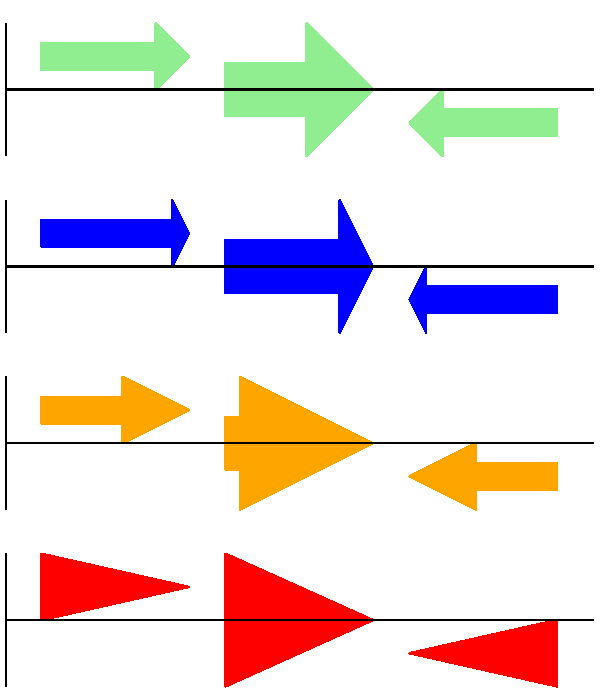
\includegraphics[width=0.8\textwidth]{images/GD_sigil_arrow_heads.png}
\caption{Simple GenomeDiagram showing arrow head options
(see Section~\ref{sec:gd_arrow_sigils})}
\label{fig:gd_sigil_arrow_heads}
\end{figure}
\end{latexonly}

Biopython 1.61 adds a new \verb|BIGARROW| sigil which always stradles
the axis, pointing left for the reverse strand or right otherwise:

\begin{verbatim}
#A large arrow straddling the axis:
gd_feature_set.add_feature(feature, sigil="BIGARROW")
\end{verbatim}

\noindent All the shaft and arrow head options shown above for the
\verb|ARROW| sigil can be used for the \verb|BIGARROW| sigil too.

\subsection{A nice example}
\label{sec:gd_nice_example}

Now let's return to the pPCP1 plasmid from \textit{Yersinia pestis biovar
Microtus}, and the top down approach used in Section~\ref{sec:gd_top_down},
but take advantage of the sigil options we've now discussed.  This time
we'll use arrows for the genes, and overlay them with strand-less features
(as plain boxes) showing the position of some restriction digest sites.

%NOTE - This *just* fits on one page in the PDF output :)
\begin{verbatim}
from reportlab.lib import colors
from reportlab.lib.units import cm
from Bio.Graphics import GenomeDiagram
from Bio import SeqIO
from Bio.SeqFeature import SeqFeature, FeatureLocation

record = SeqIO.read("NC_005816.gb", "genbank")

gd_diagram = GenomeDiagram.Diagram(record.id)
gd_track_for_features = gd_diagram.new_track(1, name="Annotated Features")
gd_feature_set = gd_track_for_features.new_set()

for feature in record.features:
    if feature.type != "gene":
        #Exclude this feature
        continue
    if len(gd_feature_set) % 2 == 0:
        color = colors.blue
    else:
        color = colors.lightblue
    gd_feature_set.add_feature(feature, sigil="ARROW",
                               color=color, label=True,
                               label_size = 14, label_angle=0)

#I want to include some strandless features, so for an example
#will use EcoRI recognition sites etc.
for site, name, color in [("GAATTC","EcoRI",colors.green),
                          ("CCCGGG","SmaI",colors.orange),
                          ("AAGCTT","HindIII",colors.red),
                          ("GGATCC","BamHI",colors.purple)]:
    index = 0
    while True:
        index  = record.seq.find(site, start=index)
        if index == -1 : break
        feature = SeqFeature(FeatureLocation(index, index+len(site)))
        gd_feature_set.add_feature(feature, color=color, name=name,
                                   label=True, label_size = 10,
                                   label_color=color)
        index += len(site)

gd_diagram.draw(format="linear", pagesize='A4', fragments=4,
                start=0, end=len(record))
gd_diagram.write("plasmid_linear_nice.pdf", "PDF")
gd_diagram.write("plasmid_linear_nice.eps", "EPS")
gd_diagram.write("plasmid_linear_nice.svg", "SVG")

gd_diagram.draw(format="circular", circular=True, pagesize=(20*cm,20*cm),
                start=0, end=len(record), circle_core = 0.5)
gd_diagram.write("plasmid_circular_nice.pdf", "PDF")
gd_diagram.write("plasmid_circular_nice.eps", "EPS")
gd_diagram.write("plasmid_circular_nice.svg", "SVG")
\end{verbatim}

\begin{htmlonly}
\noindent And the output:

\imgsrc[width=550, height=400]{images/plasmid_linear_nice.png}

\imgsrc[width=591, height=591]{images/plasmid_circular_nice.png}

\end{htmlonly}
\begin{latexonly}
\noindent The expected output is shown in Figures~\ref{fig:plasmid_linear_nice}
and~\ref{fig:plasmid_circular_nice}.
\begin{figure}[htbp]
\centering
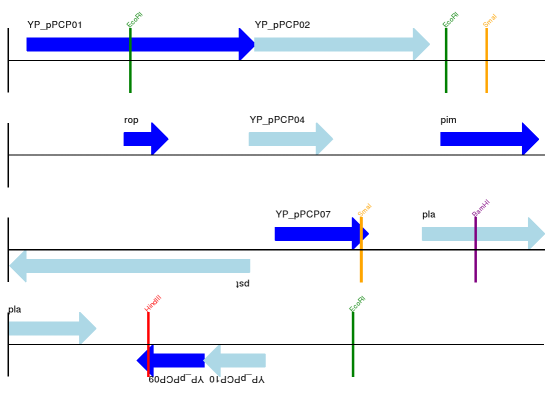
\includegraphics[width=0.8\textwidth]{images/plasmid_linear_nice.png}
\caption{Linear diagram for \textit{Yersinia pestis biovar Microtus} plasmid
pPCP1 showing selected restriction digest sites (see
Section~\ref{sec:gd_nice_example}).}
\label{fig:plasmid_linear_nice}
\end{figure}
\begin{figure}[htbp]
\centering
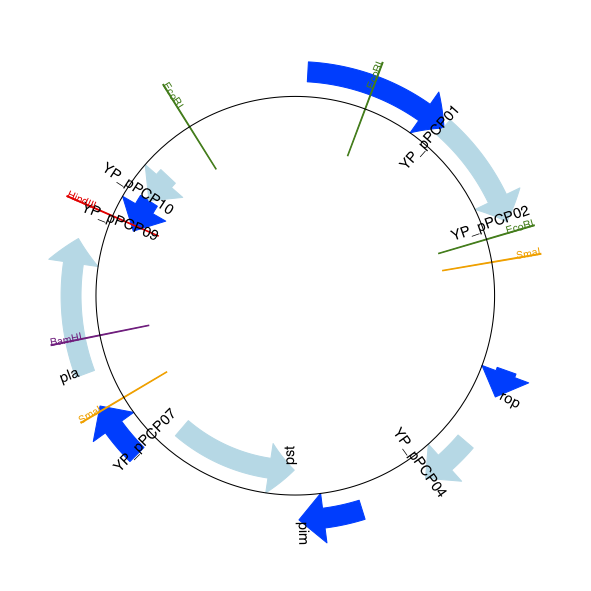
\includegraphics[width=0.8\textwidth]{images/plasmid_circular_nice.png}
\caption{Circular diagram for \textit{Yersinia pestis biovar Microtus} plasmid
pPCP1 showing selected restriction digest sites (see
Section~\ref{sec:gd_nice_example}).}
\label{fig:plasmid_circular_nice}
\end{figure}
\end{latexonly}

\subsection{Multiple tracks}
\label{sec:gd_multiple_tracks}

All the examples so far have used a single track, but you can have more than
one track -- for example show the genes on one, and repeat regions on another.
In this example we're going to show three phage genomes side by side to scale,
inspired by Figure 6 in Proux {\textit et al.} (2002) \cite{proux2002}.
We'll need the GenBank files for the following three phage:
\begin{itemize}
\item \verb|NC_002703| -- Lactococcus phage Tuc2009, complete genome ($38347$ bp)
\item \verb|AF323668| -- Bacteriophage bIL285, complete genome ($35538$ bp)
\item \verb|NC_003212| -- \textit{Listeria innocua} Clip11262, complete genome,
of which we are focussing only on integrated prophage 5 (similar length).
\end{itemize}

You can download these using Entrez if you like, see Section~\ref{sec:efetch}
for more details. For the third record we've worked out where the phage is
integrated into the genome, and slice the record to extract it (with the
features preserved, see Section~\ref{sec:SeqRecord-slicing}), and must also
reverse complement to match the orientation of the first two phage (again
preserving the features, see Section~\ref{sec:SeqRecord-reverse-complement}):

\begin{verbatim}
from Bio import SeqIO

A_rec = SeqIO.read("NC_002703.gbk", "gb")
B_rec = SeqIO.read("AF323668.gbk", "gb")
C_rec = SeqIO.read("NC_003212.gbk", "gb")[2587879:2625807].reverse_complement(name=True)
\end{verbatim}

The figure we are imitating used different colors for different gene functions.
One way to do this is to edit the GenBank file to record color preferences for
each feature - something \href{http://www.sanger.ac.uk/resources/software/artemis/}
{Sanger's Artemis editor} does, and which GenomeDiagram should understand. Here
however, we'll just hard code three lists of colors.

Note that the annotation in the GenBank files doesn't exactly match that shown
in Proux \textit{et al.}, they have drawn some unannotated genes.

\begin{verbatim}
from reportlab.lib.colors import red, grey, orange, green, brown, blue, lightblue, purple

A_colors = [red]*5 + [grey]*7 + [orange]*2 + [grey]*2 + [orange] + [grey]*11 + [green]*4 \
         + [grey] + [green]*2 + [grey, green] + [brown]*5 + [blue]*4 + [lightblue]*5 \
         + [grey, lightblue] + [purple]*2 + [grey]
B_colors = [red]*6 + [grey]*8 + [orange]*2 + [grey] + [orange] + [grey]*21 + [green]*5 \
         + [grey] + [brown]*4 + [blue]*3 + [lightblue]*3 + [grey]*5 + [purple]*2
C_colors = [grey]*30 + [green]*5 + [brown]*4 + [blue]*2 + [grey, blue] + [lightblue]*2 \
         + [grey]*5
\end{verbatim}

Now to draw them -- this time we add three tracks to the diagram, and also notice they
are given different start/end values to reflect their different lengths (this requires
Biopython 1.59 or later).

\begin{verbatim}
from Bio.Graphics import GenomeDiagram

name = "Proux Fig 6"
gd_diagram = GenomeDiagram.Diagram(name)
max_len = 0
for record, gene_colors in zip([A_rec, B_rec, C_rec], [A_colors, B_colors, C_colors]):
    max_len = max(max_len, len(record))
    gd_track_for_features = gd_diagram.new_track(1,
                            name=record.name,
                            greytrack=True,
                            start=0, end=len(record))
    gd_feature_set = gd_track_for_features.new_set()

    i = 0
    for feature in record.features:
        if feature.type != "gene":
            #Exclude this feature
            continue
        gd_feature_set.add_feature(feature, sigil="ARROW",
                                   color=gene_colors[i], label=True,
                                   name = str(i+1),
                                   label_position="start",
                                   label_size = 6, label_angle=0)
        i+=1

gd_diagram.draw(format="linear", pagesize='A4', fragments=1,
                start=0, end=max_len)
gd_diagram.write(name + ".pdf", "PDF")
gd_diagram.write(name + ".eps", "EPS")
gd_diagram.write(name + ".svg", "SVG")
\end{verbatim}

\begin{htmlonly}
\noindent The result:

\imgsrc[width=565, height=400]{images/three_track_simple.png}

\end{htmlonly}
\begin{latexonly}
\noindent The expected output is shown in Figure~\ref{fig:three_track_simple}.
\begin{figure}[htbp]
\centering
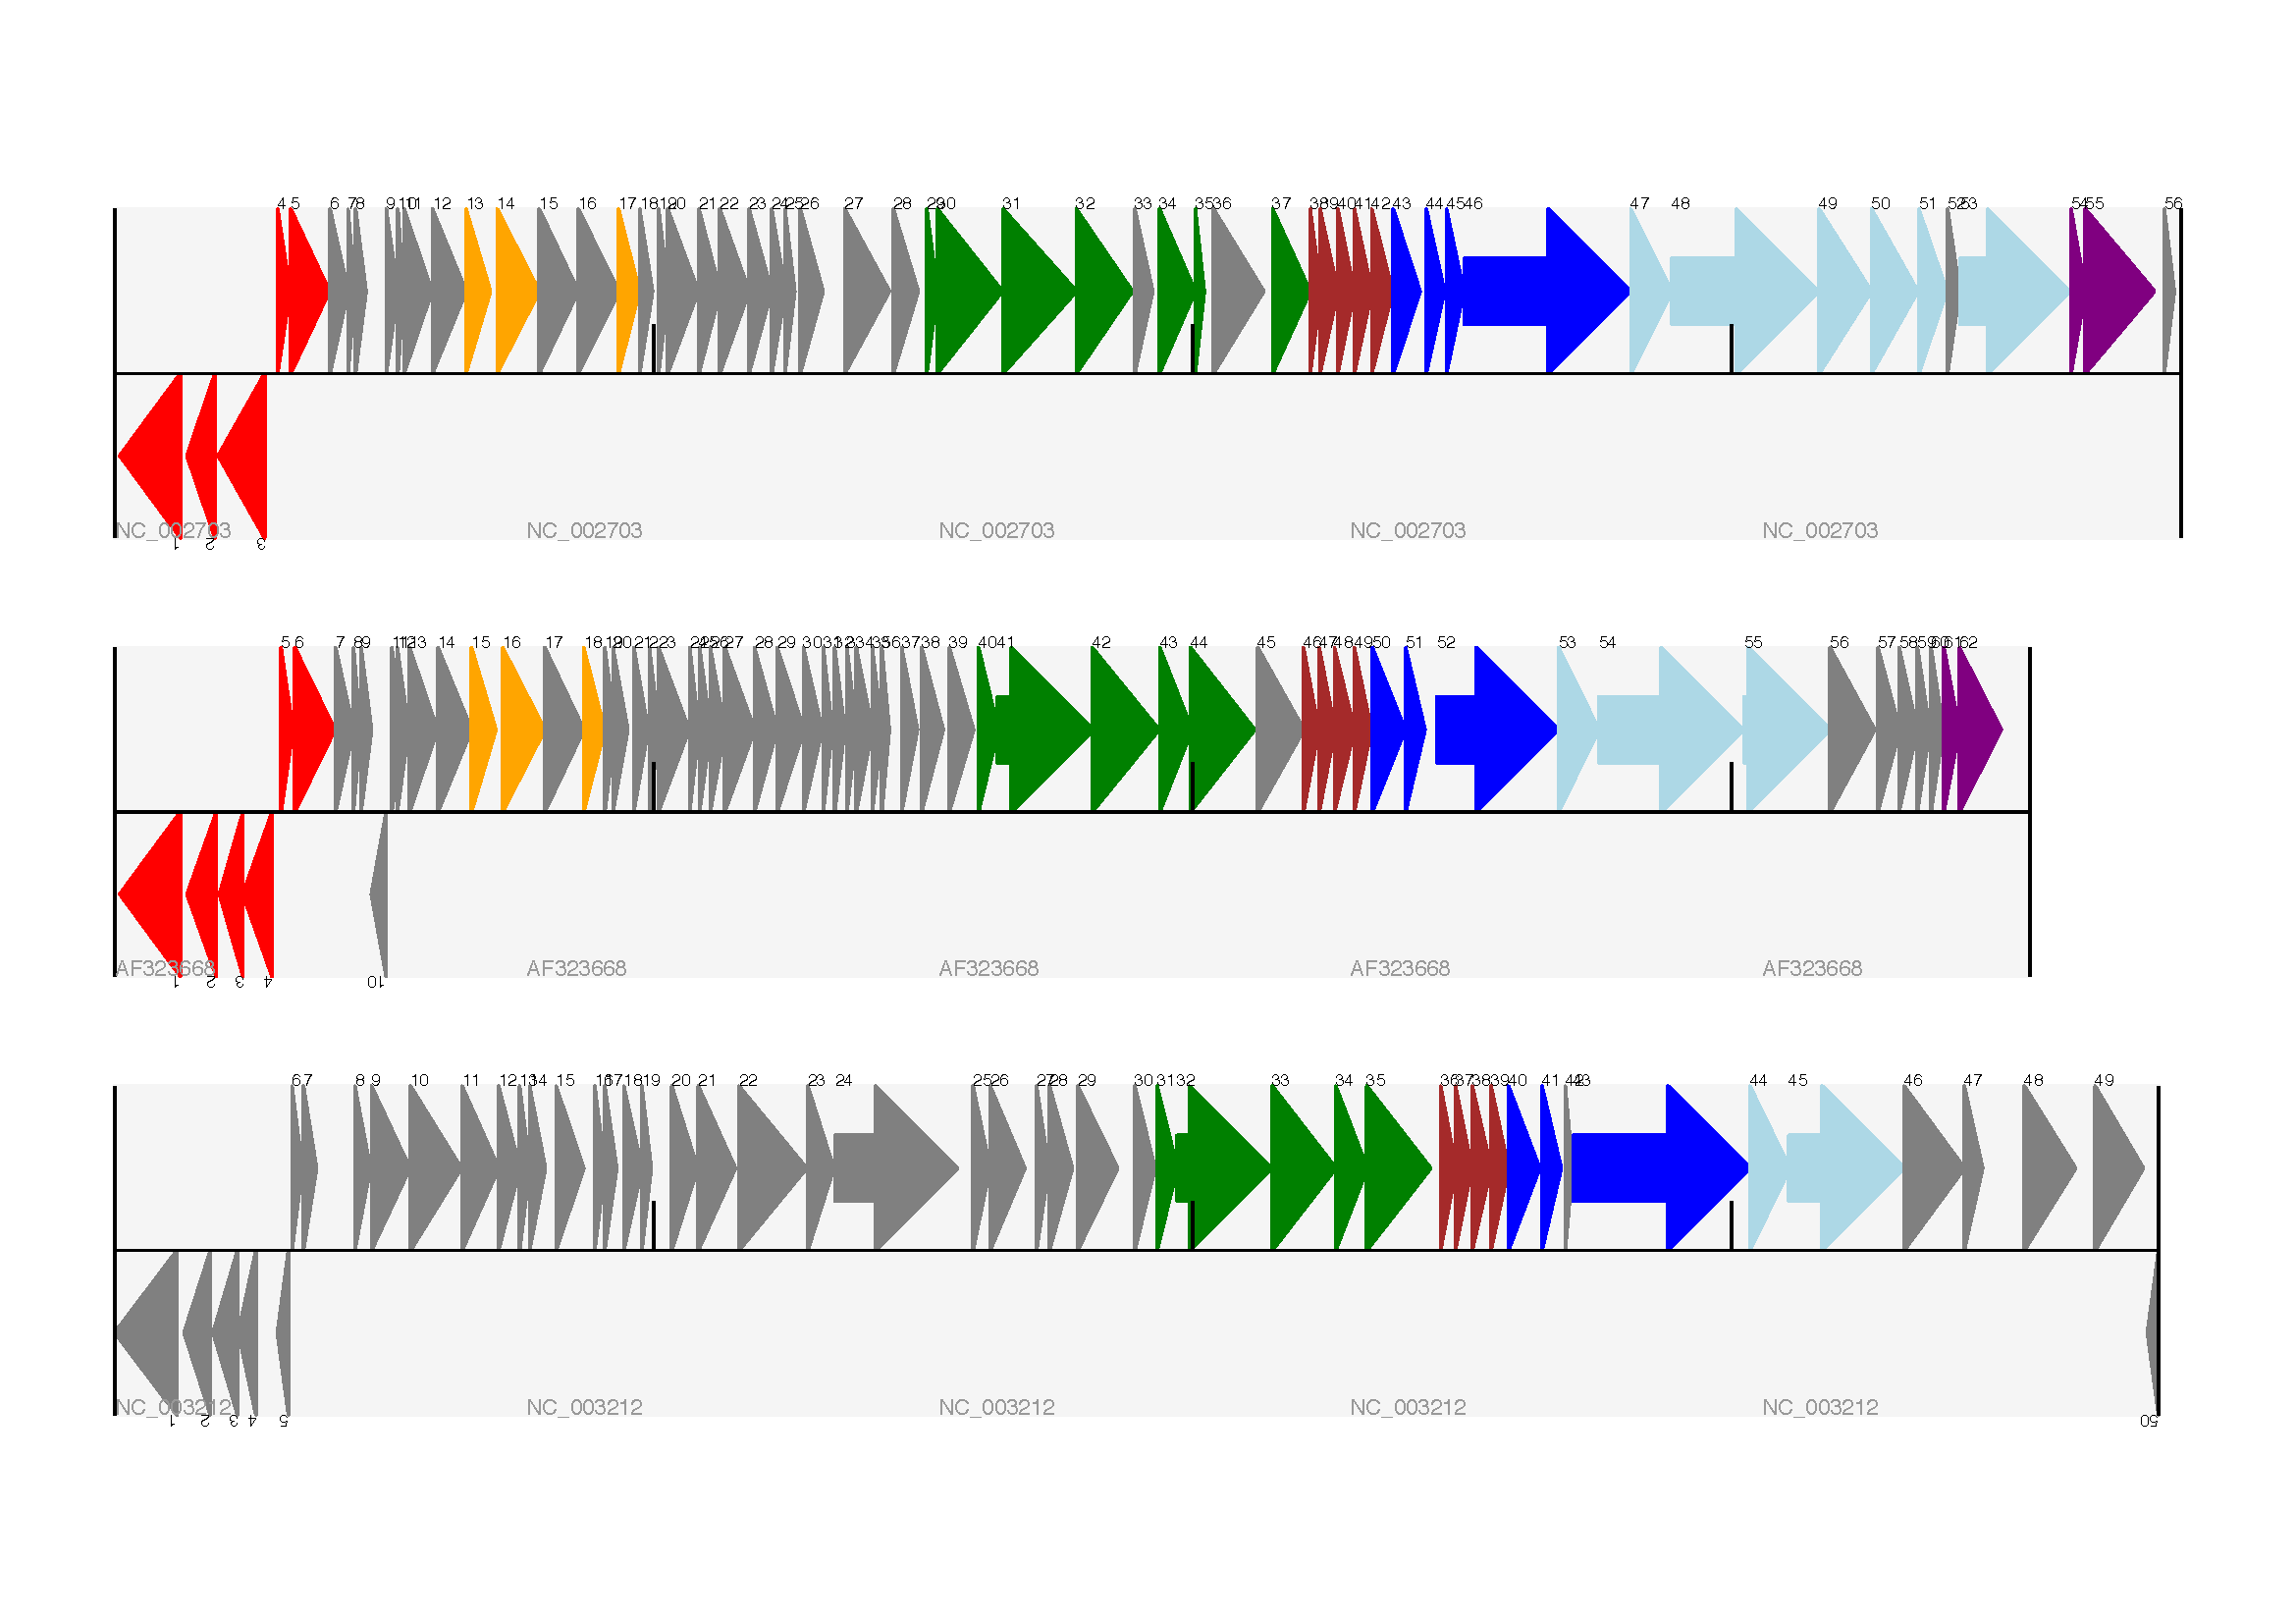
\includegraphics[width=\textwidth]{images/three_track_simple.png}
\caption{Linear diagram with three tracks for Lactococcus phage Tuc2009
(NC\_002703), bacteriophage bIL285 (AF323668), and prophage 5 from
\textit{Listeria innocua} Clip11262 (NC\_003212)
(see Section~\ref{sec:gd_multiple_tracks}).}
\label{fig:three_track_simple}
\end{figure}
\end{latexonly}
I did wonder why in the original manuscript there were no red or orange genes
marked in the bottom phage. Another important point is here the phage are
shown with different lengths - this is because they are all drawn to the same
scale (they \emph{are} different lengths).

The key difference from the published figure is they have color-coded links
between similar proteins -- which is what we will do in the next section.

\subsection{Cross-Links between tracks}
\label{sec:gd_cross_links}

Biopython 1.59 added the ability to draw cross links between tracks - both
simple linear diagrams as we will show here, but also linear diagrams split
into fragments and circular diagrams.

Continuing the example from the previous section inspired by Figure 6 from
Proux \textit{et al.} 2002 \cite{proux2002},
we would need a list of cross links between pairs of genes, along with a score
or color to use. Realistically you might extract this from a BLAST file
computationally, but here I have manually typed them in.

My naming convention continues to refer to the three phage as A, B and C.
Here are the links we want to show between A and B, given as a list of
tuples (percentage similarity score, gene in A, gene in B).

\begin{verbatim}
#Tuc2009 (NC_002703) vs bIL285 (AF323668)
A_vs_B = [
    (99, "Tuc2009_01", "int"),
    (33, "Tuc2009_03", "orf4"),
    (94, "Tuc2009_05", "orf6"),
    (100,"Tuc2009_06", "orf7"),
    (97, "Tuc2009_07", "orf8"),
    (98, "Tuc2009_08", "orf9"),
    (98, "Tuc2009_09", "orf10"),
    (100,"Tuc2009_10", "orf12"),
    (100,"Tuc2009_11", "orf13"),
    (94, "Tuc2009_12", "orf14"),
    (87, "Tuc2009_13", "orf15"),
    (94, "Tuc2009_14", "orf16"),
    (94, "Tuc2009_15", "orf17"),
    (88, "Tuc2009_17", "rusA"),
    (91, "Tuc2009_18", "orf20"),
    (93, "Tuc2009_19", "orf22"),
    (71, "Tuc2009_20", "orf23"),
    (51, "Tuc2009_22", "orf27"),
    (97, "Tuc2009_23", "orf28"),
    (88, "Tuc2009_24", "orf29"),
    (26, "Tuc2009_26", "orf38"),
    (19, "Tuc2009_46", "orf52"),
    (77, "Tuc2009_48", "orf54"),
    (91, "Tuc2009_49", "orf55"),
    (95, "Tuc2009_52", "orf60"),
]
\end{verbatim}

Likewise for B and C:

\begin{verbatim}
#bIL285 (AF323668) vs Listeria innocua prophage 5 (in NC_003212)
B_vs_C = [
    (42, "orf39", "lin2581"),
    (31, "orf40", "lin2580"),
    (49, "orf41", "lin2579"), #terL
    (54, "orf42", "lin2578"), #portal
    (55, "orf43", "lin2577"), #protease
    (33, "orf44", "lin2576"), #mhp
    (51, "orf46", "lin2575"),
    (33, "orf47", "lin2574"),
    (40, "orf48", "lin2573"),
    (25, "orf49", "lin2572"),
    (50, "orf50", "lin2571"),
    (48, "orf51", "lin2570"),
    (24, "orf52", "lin2568"),
    (30, "orf53", "lin2567"),
    (28, "orf54", "lin2566"),
]
\end{verbatim}

For the first and last phage these identifiers are locus tags, for the middle
phage there are no locus tags so I've used gene names instead. The following
little helper function lets us lookup a feature using either a locus tag or
gene name:

\begin{verbatim}
def get_feature(features, id, tags=["locus_tag", "gene"]):
    """Search list of SeqFeature objects for an identifier under the given tags."""
    for f in features:
        for key in tags:
            #tag may not be present in this feature
            for x in f.qualifiers.get(key, []):
                if x == id:
                     return f
    raise KeyError(id)
\end{verbatim}

We can now turn those list of identifier pairs into SeqFeature pairs, and thus
find their location co-ordinates. We can now add all that code and the following
snippet to the previous example (just before the \verb|gd_diagram.draw(...)|
line -- see the finished example script
\href{http://biopython.org/SRC/biopython/Doc/examples/Proux_et_al_2002_Figure_6.py}{Proux\_et\_al\_2002\_Figure\_6.py}
included in the \texttt{Doc/examples} folder of the Biopython source code)
to add cross links to the figure:

\begin{verbatim}
from Bio.Graphics.GenomeDiagram import CrossLink
from reportlab.lib import colors
#Note it might have been clearer to assign the track numbers explicitly...
for rec_X, tn_X, rec_Y, tn_Y, X_vs_Y in [(A_rec, 3, B_rec, 2, A_vs_B),
                                         (B_rec, 2, C_rec, 1, B_vs_C)]:
    track_X = gd_diagram.tracks[tn_X]
    track_Y = gd_diagram.tracks[tn_Y]
    for score, id_X, id_Y in X_vs_Y:
        feature_X = get_feature(rec_X.features, id_X)
        feature_Y = get_feature(rec_Y.features, id_Y)
        color = colors.linearlyInterpolatedColor(colors.white, colors.firebrick, 0, 100, score)
        link_xy = CrossLink((track_X, feature_X.location.start, feature_X.location.end),
                            (track_Y, feature_Y.location.start, feature_Y.location.end),
                            color, colors.lightgrey)
        gd_diagram.cross_track_links.append(link_xy)
\end{verbatim}

There are several important pieces to this code. First the \verb|GenomeDiagram| object
has a \verb|cross_track_links| attribute which is just a list of \verb|CrossLink| objects.
Each \verb|CrossLink| object takes two sets of track-specific co-ordinates (here given
as tuples, you can alternatively use a \verb|GenomeDiagram.Feature| object instead).
You can optionally supply a colour, border color, and say if this link should be drawn
flipped (useful for showing inversions).

You can also see how we turn the BLAST percentage identity score into a colour,
interpolating between white ($0\%$) and a dark red ($100\%$). In this example
we don't have any problems with overlapping cross-links. One way to tackle that
is to use transparency in ReportLab, by using colors with their alpha channel set.
However, this kind of shaded color scheme combined with overlap transparency
would be difficult to interpret.
%Again, HTML and PDF versions for the figure
\begin{htmlonly}
\noindent The result:

\imgsrc[width=565, height=400]{images/three_track_cl.png}

\end{htmlonly}
\begin{latexonly}
\noindent The expected output is shown in Figure~\ref{fig:three_track_cl}.
\begin{figure}[htbp]
\centering
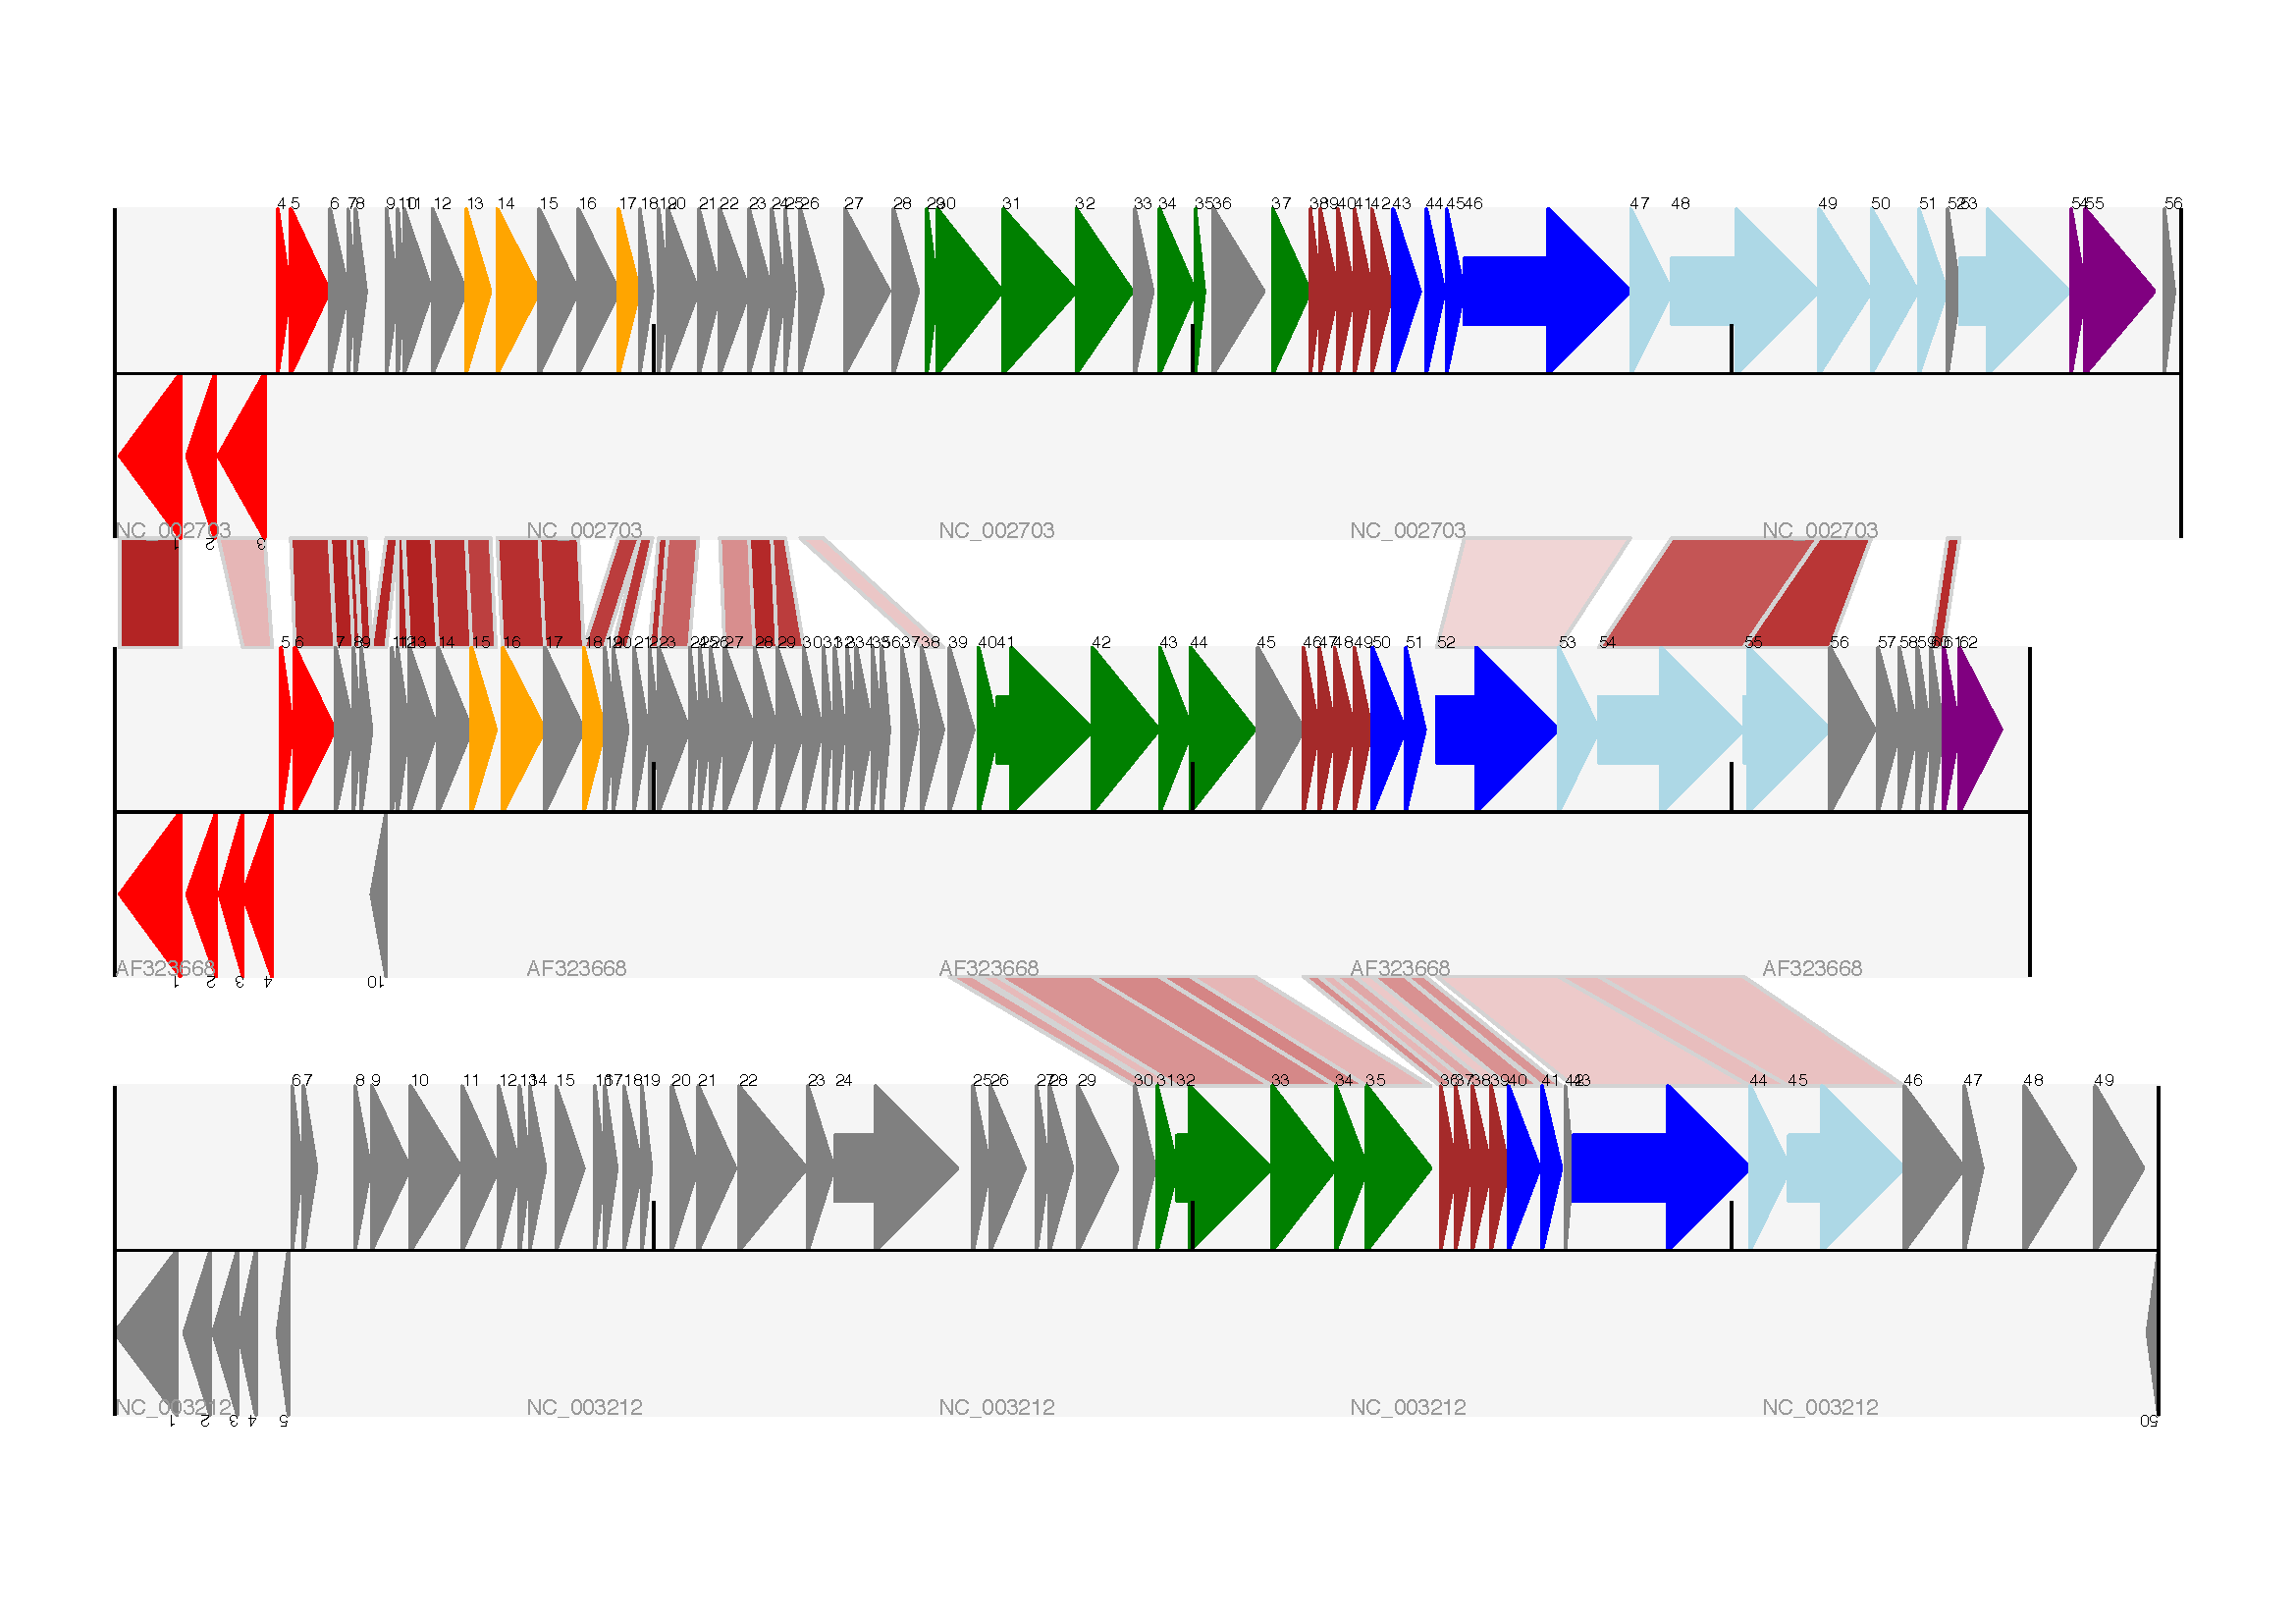
\includegraphics[width=\textwidth]{images/three_track_cl.png}
\caption{Linear diagram with three tracks for Lactococcus phage Tuc2009
(NC\_002703), bacteriophage bIL285 (AF323668), and prophage 5 from
\textit{Listeria innocua} Clip11262 (NC\_003212) plus basic cross-links
shaded by percentage identity (see Section~\ref{sec:gd_cross_links}).}
\label{fig:three_track_cl}
\end{figure}
\end{latexonly}

There is still a lot more that can be done within Biopython to help
improve this figure. First of all, the cross links in this case are
between proteins which are drawn in a strand specific manor. It can
help to add a background region (a feature using the `BOX' sigil) on the
feature track to extend the cross link. Also, we could reduce the vertical
height of the feature tracks to allocate more to the links instead -- one
way to do that is to allocate space for empty tracks. Furthermore,
in cases like this where there are no large gene overlaps, we can use
the axis-straddling \verb|BIGARROW| sigil, which allows us to further
reduce the vertical space needed for the track. These improvements
are demonstrated in the example script
\href{http://biopython.org/SRC/biopython/Doc/examples/Proux_et_al_2002_Figure_6.py}{Proux\_et\_al\_2002\_Figure\_6.py}
included in the \texttt{Doc/examples} folder of the Biopython source code.
%TODO - Add a link get the file directly (for Windows users etc).
\begin{htmlonly}
\noindent The result:

\imgsrc[width=565, height=400]{images/three_track_cl2a.png}

\end{htmlonly}
\begin{latexonly}
\noindent The expected output is shown in Figure~\ref{fig:three_track_cl2}.
\begin{figure}[htbp]
\centering
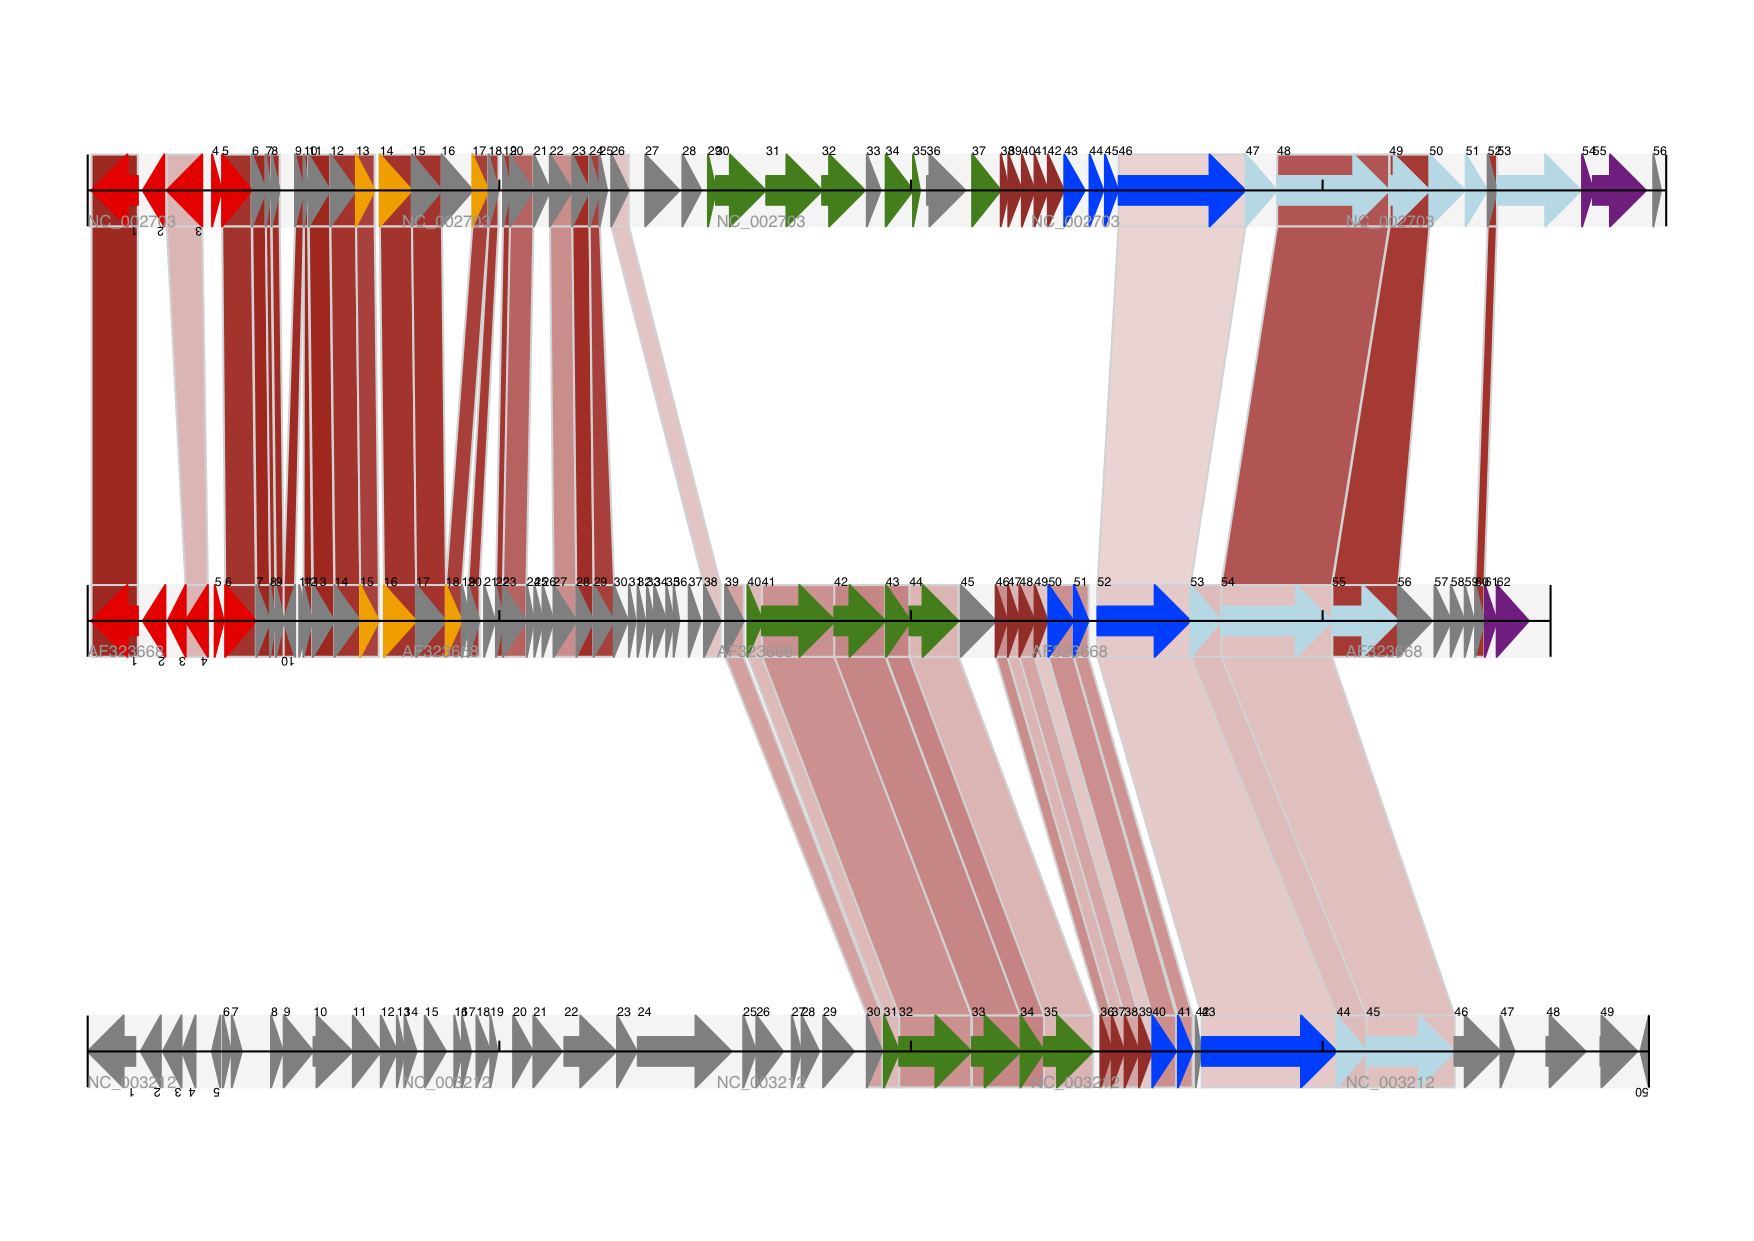
\includegraphics[width=\textwidth]{images/three_track_cl2a.png}
\caption{Linear diagram with three tracks for Lactococcus phage Tuc2009
(NC\_002703), bacteriophage bIL285 (AF323668), and prophage 5 from
\textit{Listeria innocua} Clip11262 (NC\_003212) plus cross-links
shaded by percentage identity (see Section~\ref{sec:gd_cross_links}).}
\label{fig:three_track_cl2}
\end{figure}
\end{latexonly}

Beyond that, finishing touches you might want to do manually in a vector
image editor include fine tuning the placement of gene labels, and adding
other custom annotation such as highlighting particular regions.

Although not really necessary in this example since none of the cross-links
overlap, using a transparent color in ReportLab is a very useful technique
for superimposing multiple links. However, in this case a shaded color
scheme should be avoided.

\subsection{Further options}

You can control the tick marks to show the scale -- after all every graph
should show its units, and the number of the grey-track labels.

Also, we have only used the \verb|FeatureSet| so far. GenomeDiagram also has
a \verb|GraphSet| which can be used for show line graphs, bar charts and heat
plots (e.g. to show plots of GC\% on a track parallel to the features).

These options are not covered here yet, so for now we refer you to the
\href{http://biopython.org/DIST/docs/GenomeDiagram/userguide.pdf}
%\href{http://bioinf.scri.ac.uk/lp/downloads/programs/genomediagram/userguide.pdf}
{User Guide (PDF)} included with the standalone version of GenomeDiagram (but
please read the next section first), and the docstrings.

\subsection{Converting old code}

If you have old code written using the standalone version of GenomeDiagram, and
you want to switch it over to using the new version included with Biopython then
you will have to make a few changes - most importantly to your import statements.

Also, the older version of GenomeDiagram used only the UK spellings of color and
center (colour and centre).  You will need to change to the American spellings,
although for several years the Biopython version of GenomeDiagram supported both.

For example, if you used to have:
\begin{verbatim}
from GenomeDiagram import GDFeatureSet, GDDiagram
gdd = GDDiagram("An example")
...
\end{verbatim}
you could just switch the import statements like this:
\begin{verbatim}
from Bio.Graphics.GenomeDiagram import FeatureSet as GDFeatureSet, Diagram as GDDiagram
gdd = GDDiagram("An example")
...
\end{verbatim}
and hopefully that should be enough.  In the long term you might want to
switch to the new names, but you would have to change more of your code:
\begin{verbatim}
from Bio.Graphics.GenomeDiagram import FeatureSet, Diagram
gdd = Diagram("An example")
...
\end{verbatim}
or:
\begin{verbatim}
from Bio.Graphics import GenomeDiagram
gdd = GenomeDiagram.Diagram("An example")
...
\end{verbatim}

If you run into difficulties, please ask on the Biopython mailing list for
advice. One catch is that we have not included the old module
\verb|GenomeDiagram.GDUtilities| yet.  This included a number of
GC\% related functions, which will probably be merged under
\verb|Bio.SeqUtils| later on.
%TODO - Deal with GenomeDiagram.GDUtilities

\section{Chromosomes}

The \verb|Bio.Graphics.BasicChromosome| module allows drawing of chromosomes.
There is an example in Jupe \textit{et al.} (2012) \cite{jupe2012}
(open access) using colors to highlight different gene families.

\subsection{Simple Chromosomes}
Here is a very simple example - for which we'll use \textit{Arabidopsis thaliana}.

\begin{latexonly}
\begin{figure}[p]
\centering
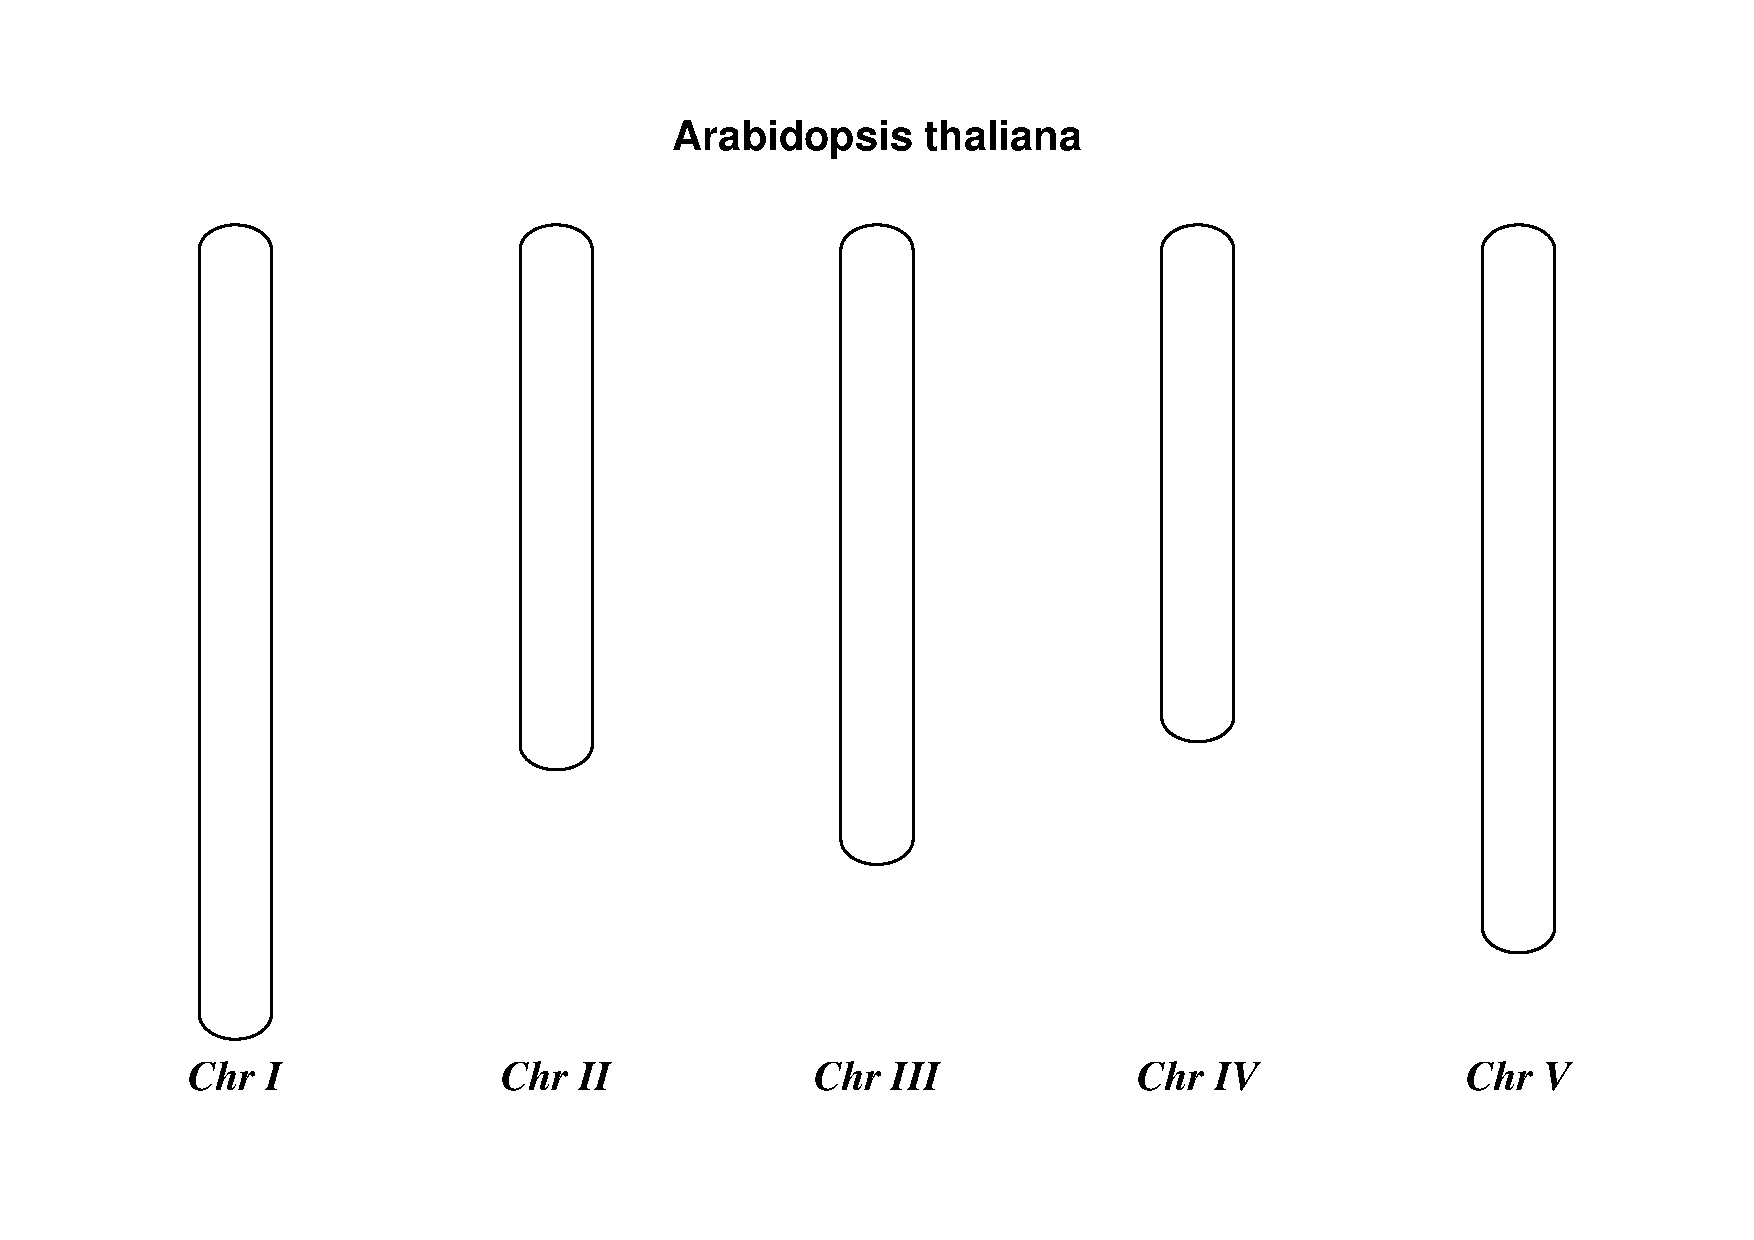
\includegraphics[scale=0.45]{images/simple_chrom.pdf}
\caption{Simple chromosome diagram for \textit{Arabidopsis thaliana}.}
\label{fig:simplechromosome}
\end{figure}
\begin{figure}[p]
\centering
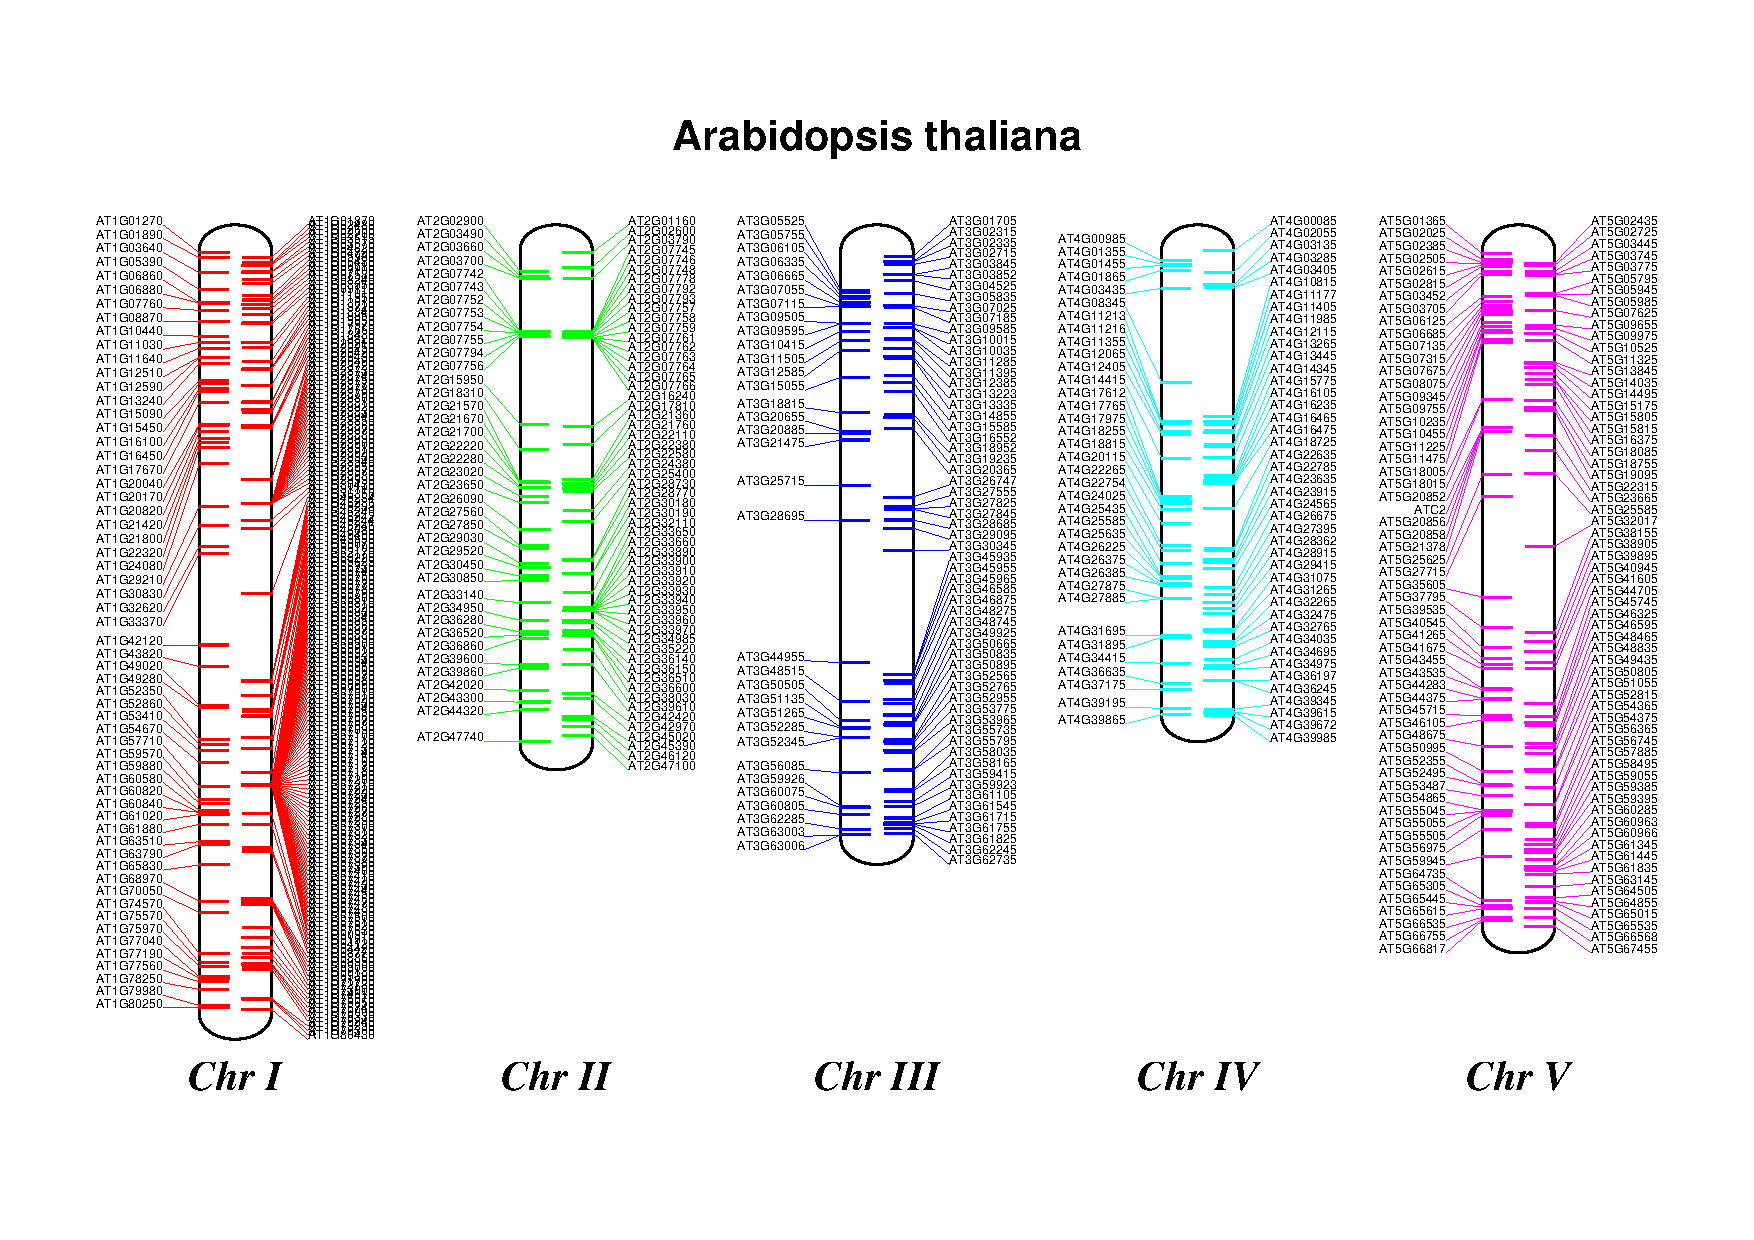
\includegraphics[scale=0.45]{images/tRNA_chrom.pdf}
\caption{Chromosome diagram for \textit{Arabidopsis thaliana} showing tRNA genes.}
\label{fig:trnachromosome}
\end{figure}
\end{latexonly}

You can skip this bit, but first I downloaded the five sequenced chromosomes
from the NCBI's FTP site
\url{ftp://ftp.ncbi.nlm.nih.gov/genomes/Arabidopsis_thaliana} and then parsed
them with \verb|Bio.SeqIO| to find out their lengths.  You could use the
GenBank files for this, but it is faster to use the FASTA files for the
whole chromosomes:

\begin{verbatim}
from Bio import SeqIO
entries = [("Chr I", "CHR_I/NC_003070.fna"),
           ("Chr II", "CHR_II/NC_003071.fna"),
           ("Chr III", "CHR_III/NC_003074.fna"),
           ("Chr IV", "CHR_IV/NC_003075.fna"),
           ("Chr V", "CHR_V/NC_003076.fna")]
for (name, filename) in entries:
   record = SeqIO.read(filename,"fasta")
   print(name, len(record))
\end{verbatim}

\noindent This gave the lengths of the five chromosomes, which we'll now use in
the following short demonstration of the \verb|BasicChromosome| module:

\begin{verbatim}
from reportlab.lib.units import cm
from Bio.Graphics import BasicChromosome

entries = [("Chr I", 30432563),
           ("Chr II", 19705359),
           ("Chr III", 23470805),
           ("Chr IV", 18585042),
           ("Chr V", 26992728)]

max_len = 30432563 #Could compute this
telomere_length = 1000000 #For illustration

chr_diagram = BasicChromosome.Organism()
chr_diagram.page_size = (29.7*cm, 21*cm) #A4 landscape

for name, length in entries:
    cur_chromosome = BasicChromosome.Chromosome(name)
    #Set the scale to the MAXIMUM length plus the two telomeres in bp,
    #want the same scale used on all five chromosomes so they can be
    #compared to each other
    cur_chromosome.scale_num = max_len + 2 * telomere_length

    #Add an opening telomere
    start = BasicChromosome.TelomereSegment()
    start.scale = telomere_length
    cur_chromosome.add(start)

    #Add a body - using bp as the scale length here.
    body = BasicChromosome.ChromosomeSegment()
    body.scale = length
    cur_chromosome.add(body)

    #Add a closing telomere
    end = BasicChromosome.TelomereSegment(inverted=True)
    end.scale = telomere_length
    cur_chromosome.add(end)

    #This chromosome is done
    chr_diagram.add(cur_chromosome)

chr_diagram.draw("simple_chrom.pdf", "Arabidopsis thaliana")
\end{verbatim}

This should create a very simple PDF file, shown
\begin{htmlonly}
here:

%The blank lines above and below are important to trigger paragraph breaks
\imgsrc[width=650, height=460]{images/simple_chrom.png}

\end{htmlonly}
\begin{latexonly}
in Figure~\ref{fig:simplechromosome}.
\end{latexonly}
This example is deliberately short and sweet. The next example shows the
location of features of interest.

\subsection{Annotated Chromosomes}

Continuing from the previous example, let's also show the tRNA genes.
We'll get their locations by parsing the GenBank files for the five
\textit{Arabidopsis thaliana} chromosomes. You'll need to download these
files from the NCBI FTP site
\url{ftp://ftp.ncbi.nlm.nih.gov/genomes/Arabidopsis_thaliana},
and preserve the subdirectory names or edit the paths below:

\begin{verbatim}
from reportlab.lib.units import cm
from Bio import SeqIO
from Bio.Graphics import BasicChromosome

entries = [("Chr I", "CHR_I/NC_003070.gbk"),
           ("Chr II", "CHR_II/NC_003071.gbk"),
           ("Chr III", "CHR_III/NC_003074.gbk"),
           ("Chr IV", "CHR_IV/NC_003075.gbk"),
           ("Chr V", "CHR_V/NC_003076.gbk")]

max_len = 30432563 #Could compute this
telomere_length = 1000000 #For illustration

chr_diagram = BasicChromosome.Organism()
chr_diagram.page_size = (29.7*cm, 21*cm) #A4 landscape

for index, (name, filename) in enumerate(entries):
    record = SeqIO.read(filename,"genbank")
    length = len(record)
    features = [f for f in record.features if f.type=="tRNA"]
    #Record an Artemis style integer color in the feature's qualifiers,
    #1 = Black, 2 = Red, 3 = Green, 4 = blue, 5 =cyan, 6 = purple
    for f in features: f.qualifiers["color"] = [index+2]

    cur_chromosome = BasicChromosome.Chromosome(name)
    #Set the scale to the MAXIMUM length plus the two telomeres in bp,
    #want the same scale used on all five chromosomes so they can be
    #compared to each other
    cur_chromosome.scale_num = max_len + 2 * telomere_length

    #Add an opening telomere
    start = BasicChromosome.TelomereSegment()
    start.scale = telomere_length
    cur_chromosome.add(start)

    #Add a body - again using bp as the scale length here.
    body = BasicChromosome.AnnotatedChromosomeSegment(length, features)
    body.scale = length
    cur_chromosome.add(body)

    #Add a closing telomere
    end = BasicChromosome.TelomereSegment(inverted=True)
    end.scale = telomere_length
    cur_chromosome.add(end)

    #This chromosome is done
    chr_diagram.add(cur_chromosome)

chr_diagram.draw("tRNA_chrom.pdf", "Arabidopsis thaliana")
\end{verbatim}

It might warn you about the labels being too close together - have a look
at the forward strand (right hand side) of Chr I, but it should create a
colorful PDF file, shown
\begin{htmlonly}
here:

%The blank lines above and below are important to trigger paragraph breaks
\imgsrc[width=650, height=460]{images/tRNA_chrom.png}

\end{htmlonly}
\begin{latexonly}
in Figure~\ref{fig:simplechromosome}.
\end{latexonly}

